\documentclass[12pt, a4paper, twoside]{book}
\usepackage[utf8]{inputenc} % Aceptar diferentes tipos de codificación de caracteres de entrada (en este caso usamos la codificación Unicode UTF-8)
%\usepackage{natbib}
\usepackage{listings}
\usepackage{eurosym}
\usepackage[spanish]{babel}
\usepackage{titlesec}
\usepackage{graphicx} % Soporte aumentado para gráficos 
\usepackage{float}
\usepackage{hyperref} % Para manejar referencias cruzadas. P.ej. añadir hiperenlaces al índice
\usepackage{caption}
\usepackage{setspace}
\usepackage{color}
\usepackage[a4paper, top=3.5cm, bottom=3.5cm, left=3cm, right=3cm]{geometry}
\spacing{1.5}
\setcounter{secnumdepth}{4}
\setlength{\parindent}{12pt}
\titleformat{\paragraph}
{\normalfont\normalsize\bfseries}{\theparagraph}{1em}{}
\titlespacing*{\paragraph}
{0pt}{3.25ex plus 1ex minus .2ex}{1.5ex plus .2ex}

%\usepackage{inconsolata}
%
%\usepackage[T1]{fontenc}
%
\definecolor{dkgreen}{rgb}{0,0.6,0}
\definecolor{gray}{rgb}{0.5,0.5,0.5}
\definecolor{mauve}{rgb}{0.58,0,0.82}

\lstset{frame=tb,
	language=Java,
	aboveskip=3mm,
	belowskip=3mm,
	showstringspaces=false,
	columns=flexible,
	basicstyle={\small\ttfamily},
	numbers=none,
	numberstyle=\tiny\color{gray},
	keywordstyle=\color{blue},
	commentstyle=\color{dkgreen},
	stringstyle=\color{mauve},
	breaklines=true,
	breakatwhitespace=true,
	tabsize=3
}


\begin{document}	
	
	\thispagestyle{empty} 	
	%%%%%%%%%%%%%%%%%%%%%%%%%%%%%%%%%%%%%%%%%%%%%%%%%%%%%%%%%%%%%%%%%%%%%%%%%%%%%%%%
	% PORTADA
	%%%%%%%%%%%%%%%%%%%%%%%%%%%%%%%%%%%%%%%%%%%%%%%%%%%%%%%%%%%%%%%%%%%%%%%%%%%%%%%%
	
	\begin{center}		
		
\includegraphics[width=15cm]{Imagenes/Simbolo_logo_UDC.png}
	\end{center}
	
	% Lista de tamaños: \Huge, \huge, \LARGE, \Large, \large, \small, \footnotesize, \tiny
	\vspace{2cm}
	
	\begin{center}		
		{\textbf{ FACULTADE DE INFORMÁTICA}}
		
		\vspace{1cm}
		\LARGE{ TRABALLO FIN DE MÁSTER }	\\
		\LARGE{ MÁSTER UNIVERSITARIO EN INGENIERÍA INFORMÁTICA } \\
		\vspace{1cm}	
		\LARGE{\textbf{ Aplicación web para a xestión de menús domésticos con servizos nutricionais : Eat Fit Week! }}
	\end{center}
	
	\vspace{2cm}
	\hfill \textbf{Autor: \textit{Elías Ferreiro Borreiros}}
	
	
	\hfill \textbf{Director: \textit{Juan José Sánchez Penas}} 
	
	
	\hfill A Coruña, Agosto, 2019					
	
	\clearpage
	
	\begin{center}
		\LARGE{\textbf{ RESUMEN }}	
	\end{center}
	Hoy en día, con el cambio en los estilos de vida de las personas y tendiendo hacia unas costumbres más sedentarias, hay una mayor necesidad de enfocarse en una dieta equilibrada y saludable.
	Para ello, se han desarrollado muchos sistemas webs y móviles para la gestión de comidas y de sus valores nutricionales.	Sin embargo, analizando esos sistemas, vemos que tienen un error en su planteamiento al inundar a los usuarios con formularios sobrecargados y repletos de información innecesaria. 
	El otro problema principal de estos sistemas es la cantidad exagerada de trabajo manual que debe hacer el usuario antes de poder disfrutar de la funcionalidad principal. 
	
	Para resolver todo esto, hemos decidido plantear el desarrollo de una aplicación que solvente estos problemas y ofrezca una funcionalidad que no disponen los competidores : el análisis nutricional dinámico de las comidas planificadas para la semana configurable por el usuario. está sobrepasando.
	
	A mayores permitiremos la gestión de las entidades necesarias para esta planificación: ingredientes, platos, menús ... 
	Esto se hará siguiendo la filosofía inicial del proyecto: simplificar la entrada lo más posible y disminuir el esfuerzo requerido por el usuario. 
	Para esto llamaremos a servicios externos que nos permitirán estimar las características nutricionales de los ingredientes de forma que el usuario no tendrá que indicar esos datos y permitiremos con cada registro de usuario el alta automática de unos ingredientes base utilizables en la mayoría de recetas que agilizarán la configuración necesaria de un nuevo perfil para permitir disfrutar al máximo al usuario de las funcionalidades realmente importantes desde el momento más temprano posible.
	
	\clearpage
	
	\textbf{Título:} Aplicación web para a xestión de menús domésticos con servizos nutricionais
	\\
	\textbf{Autor:} Elías Ferreiro Borreiros
	\\
	\textbf{Tutor/Director:} Juan José Sánchez Penas
	
	
	\textbf{Palabras clave:} Java EE, POJO, Maven, Angular JS, Spring, Hibernate, Web, MySQL, Tarea, Lista, Contexto, Cliente - Servidor, Food, Planning, Management, Scrum. 
	
	
	\renewcommand{\contentsname}{Índice de contenidos}
	\renewcommand{\listfigurename}{Índice de figuras}
	\renewcommand{\listtablename}{Índice de tablas}
	
	\tableofcontents % indice de contenidos
	
	\listoffigures % indice de figuras
	
	\listoftables % indice de tablas
	
	\clearpage
	
	\chapter{PRUEBAS}
	\section{Introducción}
	Para verificar que el software desarrollado funciona correctamente, es sometido a varias pruebas.
	\section{Pruebas Unitarias}
	El objetivo de estas pruebas es verificar que el funcionamiento de cada módulo por separado es correcto, verificando que para diversas entradas en cada método, las salidas son las esperadas. Se intenta centrarse en probar los casos más característicos susceptibles de producir algún error. También se contemplan casos de prueba sobre operaciones que implican algún tipo de error como respuesta, por ejemplo, intentar obtener una menú que no existe. Para realizar dichas pruebas, se utilizan las librerías proporcionadas por JUnit, las cuales están integradas con Eclipse y permiten ejecutar casos de prueba de forma controlada, mostrando los casos superados y las pruebas que han detectado algún error. Con la utilización de Mockito se agiliza y se facilita bastante la labor de creación de tests unitarios ya que nos permite utilizar datos mockeados en la información de componentes externos de cada método que probamos unitariamente.
	\begin{figure}[H]
		\centering
		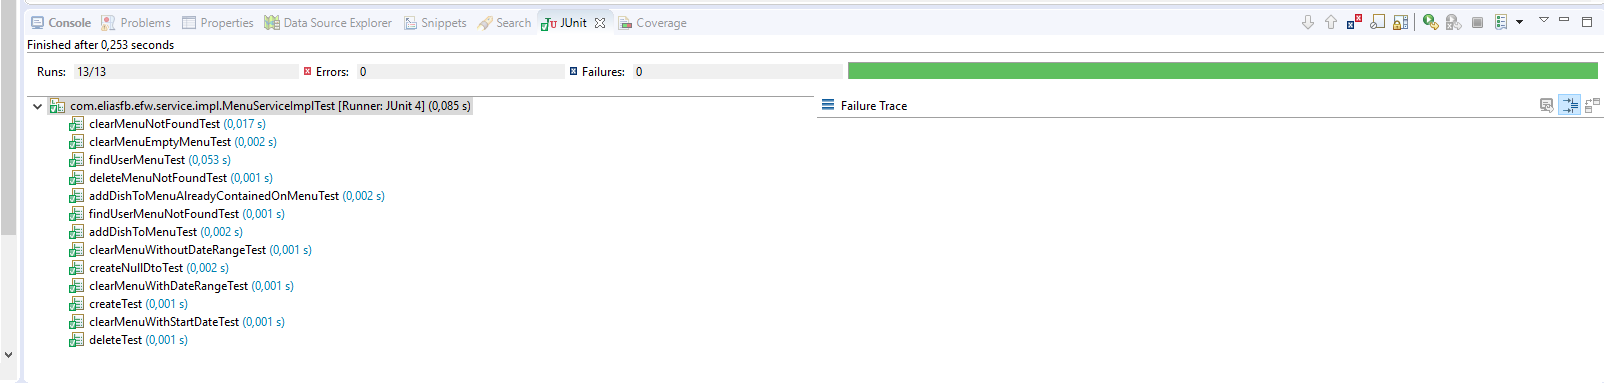
\includegraphics[width=15cm]{Imagenes/Tests.png}
		\caption{Tests Unitarios}\label{Tests Unitarios}
	\end{figure}
	\section{Cobertura}
	Utilizamos el plugin de Eclipse, Eclemma, para analizar el nivel de cobertura obtenido con las pruebas unitarias.
	Como se puede ver en la figura, el nivel de cobertura obtenido es bastante alto en la mayoría de los casos ya que, durante el desarrollo de las pruebas unitarias, nos hemos centrado en el recorrido de todas las posibles ramas del código, llamando a las operaciones con argumentos de todos los rangos de valores posibles.
	\begin{figure}[H]
		\centering
		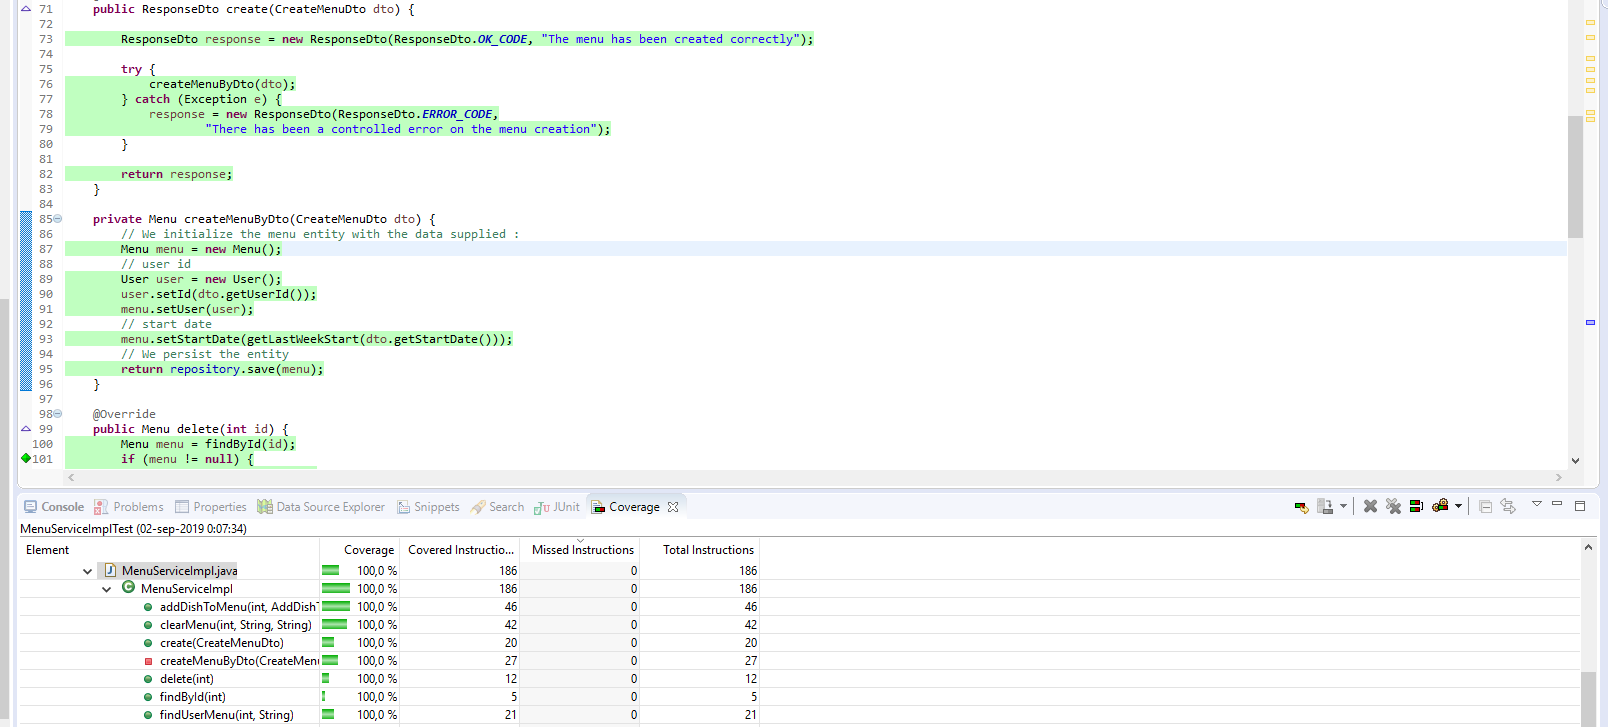
\includegraphics[width=15cm]{Imagenes/Cobertura.png}
		\caption{Cobertura}\label{Cobertura}
	\end{figure}
	\section{Pruebas de Usuario}
	El ser un sistema de gran aplicabilidad y tener un público tan variado nos ha permitido organizar sesiones de prueba y feedback con potenciales usuarios en diferentes etapas del desarrollo del sistema.
	Esto nos ha dado dos ventajas:
	\begin{itemize}
		\item Pruebas de integración de backend y frontend sobre el sistema en usos habituales del sistema
		\item Obtención de nuevos requisitos no concebidos en la planificación inicial. Requisitos a mayores obtenidos de estas sesiones han sido: Hacer las comidas semanales configurables (Desayuno, Comida, Merienda ...) tanto su número como sus nombres y Añadición de plato a primer hueco disponible de menú permitido
	\end{itemize}
	Estas pruebas a mayores añaden verificación de calidad sobre el sistema en un uso ``real'' de la aplicación.
	
\end{document}

